%*************************************************************************************************************************
\section{Uncertainty Quantification in Nuclear Engineering Thermal-Hydraulics}\label{sec:intro_uncertainty_quantification}
%*************************************************************************************************************************

% Introductory Paragraph
Before continuing the discussion of uncertainty analysis of code predictions, this section defines some additional terminologies to avoid later confusion.

The notion of \emph{simulator} introduced in Section~\ref{sec:intro_computer_simulation} is depicted in a more generic way, as an input/output model in Fig.~\ref{fig:ch1_simulator_io}.
\begin{figure}[bth]	
	\centering
	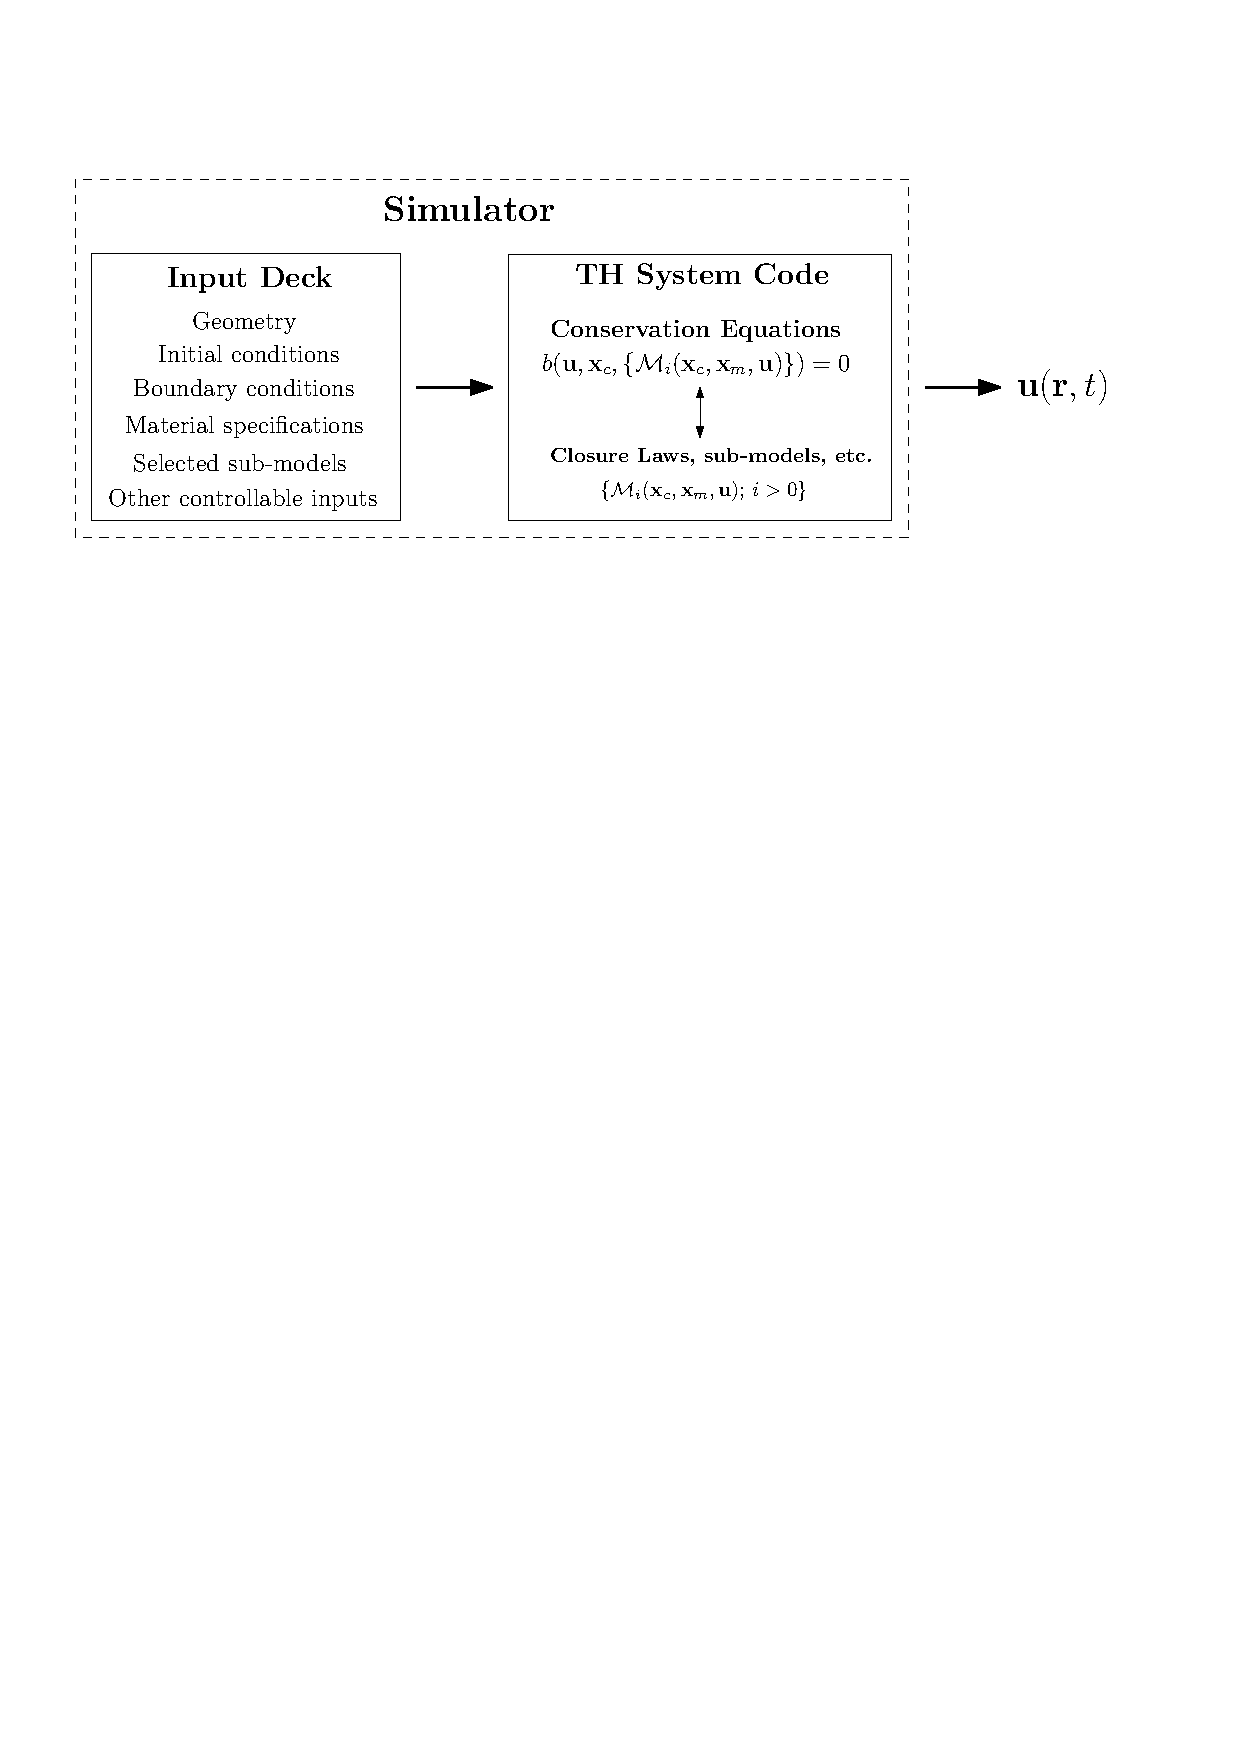
\includegraphics[width=\textwidth]{../figures/chapter1/figures/simulator_io}
	\caption[Simplified illustration of a simulator as an input/output model.]{Simplified illustration of a simulator as an input/output model.}
	\label{fig:ch1_simulator_io}
\end{figure}

The input deck defines a specific problem (i.e., system) of interest and can be seen as the input of \gls[hyper=false]{th} codes.
It includes the geometrical configuration (i.e., the nodalization), the material and fluid involved, the initial and boundary conditions, and possibly the settings for the numerical solver.
\marginpar{Controllable inputs and model parameters}
Some of these specifications (such as the boundary conditions) are parametrized and constitutes \emph{controllable inputs} denoted by $\bm{x}_c$.
The simulator is to be run for a given controllable input value\footnote{Later on, \emph{controllable} inputs correspond to the parameters whose counterparts in a physical experiment which can be controlled by the experimentalist.}.
The conservation equations of the code are closed with additional set of closure laws (and other sub-models) $\mathcal{M}_i(\bm{x}_c, \bm{x}_m, \bm{u})$.
These closure laws are, in turn, parametrized by a set of model specific parameters denoted by $\bm{x}_m$ which are referred to as the \emph{physical model parameters}.
Both the controllable inputs and the physical model parameters are considered by the code as \emph{inputs}.
 
Specifying the input deck, as far as the user is concerned, completely defines the problem and the code solves the conservation equations $b$ to estimate the physical variables $\mathbf{u}(\bm{r}, t)$ (where $\bm{r}$ and $t$ denote space and time variables, respectively) associated with the fluid flow and heat structure (e.g., fluid pressure, temperature, wall temperature, etc.).
These ``raw'' outputs are further post-processed to obtain relevant \glspl[hyper=false]{qoi} of relevance to the problem at hand (e.g., max. temperature, max. pressure, onset time, etc.).

%--------------------------------------------------------------------------
\subsection{Forward Uncertainty Quantification}\label{sub:intro_uq_forward}
%--------------------------------------------------------------------------

% Best-estimate, limitation
Best-estimate analysis attempts to describe as realistically as possible the behaviors of the physical processes that occur during a plant transient.
And yet, neither complete understanding nor enough data is available to adequately simulate these complex physical phenomena.
Simplifying assumptions, approximations, and expert judgments remain to some degree unavoidable to have a complete analysis.

% Best-estimate, plus uncertainty
Hence, best-estimate analysis has to be complemented with uncertainty analysis.
\marginpar{Best-estimate plus uncertainty}
The ultimate goal of uncertainty analysis is to associate code prediction a with its uncertainty.
These combined quantities are then compared with safety limits (e.g., \gls[hyper=false]{pct}) to check whether the limits still fall outside the uncertainty band of the code prediction.

% Source of possible uncertainties
There are several known sources of uncertainty that render the prediction on $\bm{u}(\mathbf{r},t)$ and its derived quantities uncertain.
\marginpar{Sources of uncertainty}
The the sources of primary interest in the present research are:
\begin{enumerate}

	\item \emph{Uncertainty associated with the controllable inputs}.
	In the case of a controlled experiment, controllable inputs are observed and \emph{controlled} for.
	However, their observations might contain errors due to instrument imprecision or inherent variability. 
	When simulating a real accident scenario in a plant,
  plant parameters prior to the accident scenario can also be measured and constitute uncertain controllable inputs.
  In addition, parameters defining the accident scenario, such as the break size in a \gls[hyper=false]{loca}, or the availability and performance of safety systems can also be treated as uncertain controllable inputs \cite{IAEA2002}.

  \item \emph{Uncertainty associated with the physical model parameters}.
	The value of the physical model parameters are often not known a priori.
	As such the uncertainties are epistemic.
	They can either be estimated using data from a calibration experiment or by expert judgment.
	
  \item \emph{Uncertainty associated with the physical models}.
	The physical models themselves are still approximations, even with perfectly known model parameters.
	If derived in a fully mechanistic manner, some important processes might be unaccounted for due to the inherent complexity and lack of knowledge (i.e., the case of \emph{missing physics}).
	On the contrary, if derived fully empirically, models might be derived separately for different elementary processes, while in the applications of the code multiple such models are used in concert.
	Despite each being validated, it is fair to question the validity of models used in an ensemble.
	Any of the two points tends to cause a systematic bias on the code prediction, the extend of which is unknown and uncertain.
	As a result, this source of uncertainty is referred to as model \emph{bias}, \emph{inadequacy}, or \emph{discrepancy}.

\end{enumerate}

% Forward uncertainty quantification, Inputs as random variables
In uncertainty analysis, the controllable inputs and physical model parameters are modeled as random variables ($\bm{\mathcal{X}}_c$ and $\bm{\mathcal{X}}_m$, respectively) equipped with \glspl[hyper=false]{pdf}.
\marginpar{Forward uncertainty quantification}
By transforming the random variable inputs, the simulator output becomes random variable as well
\begin{equation*}
	\bm{\mathcal{U}}(\bm{r}, t) = f(\bm{\mathcal{X}}_c, \bm{\mathcal{X}}_m;\bm{r}, t)
\end{equation*}
where $f$ represents the simulator as a mathematical function.
The \gls[hyper=false]{qoi} related to the random outputs can be summarized by different integral quantities.
For instance, the mean of a \gls[hyper=false]{qoi} given by function $g$ is
\begin{equation*}
	\mathbb{E}[g] = \int\limits_{\mathbf{X}_c,\mathbf{X}_m} g(f(\bm{x}_c, \bm{x}_m;\bm{r}, t)) \, p(\bm{x}_c, \bm{x}_m) \, d\bm{x}_c \, d\bm{x}_m
\end{equation*}
where $p(\bm{x}_c, \bm{x}_m)$ denotes the joint \gls[hyper=false]{pdf} for the input parameters.

Using \gls[hyper=false]{mc} techniques, samples are generated from their respective distributions and are used to run the code multiple times.
Afterward, the resulting code outputs (raw or post-processed), are summarized to obtain the uncertainty measure of the prediction.
In other words, the uncertainties in the controllable inputs and physical model parameters are \emph{propagated forward} through the code to quantify the uncertainty of the predictions as shown in Fig.~\ref{fig:ch1_simulator_uq_forward}.
The practice of propagating parametric uncertainty by \gls[hyper=false]{mc} is widely accepted in the nuclear engineering thermal-hydraulics community \cite{Lellouche1990,Glaeser1994,Wallis2007,Glaeser2008}.
\begin{figure}[!bth]	
	\centering
	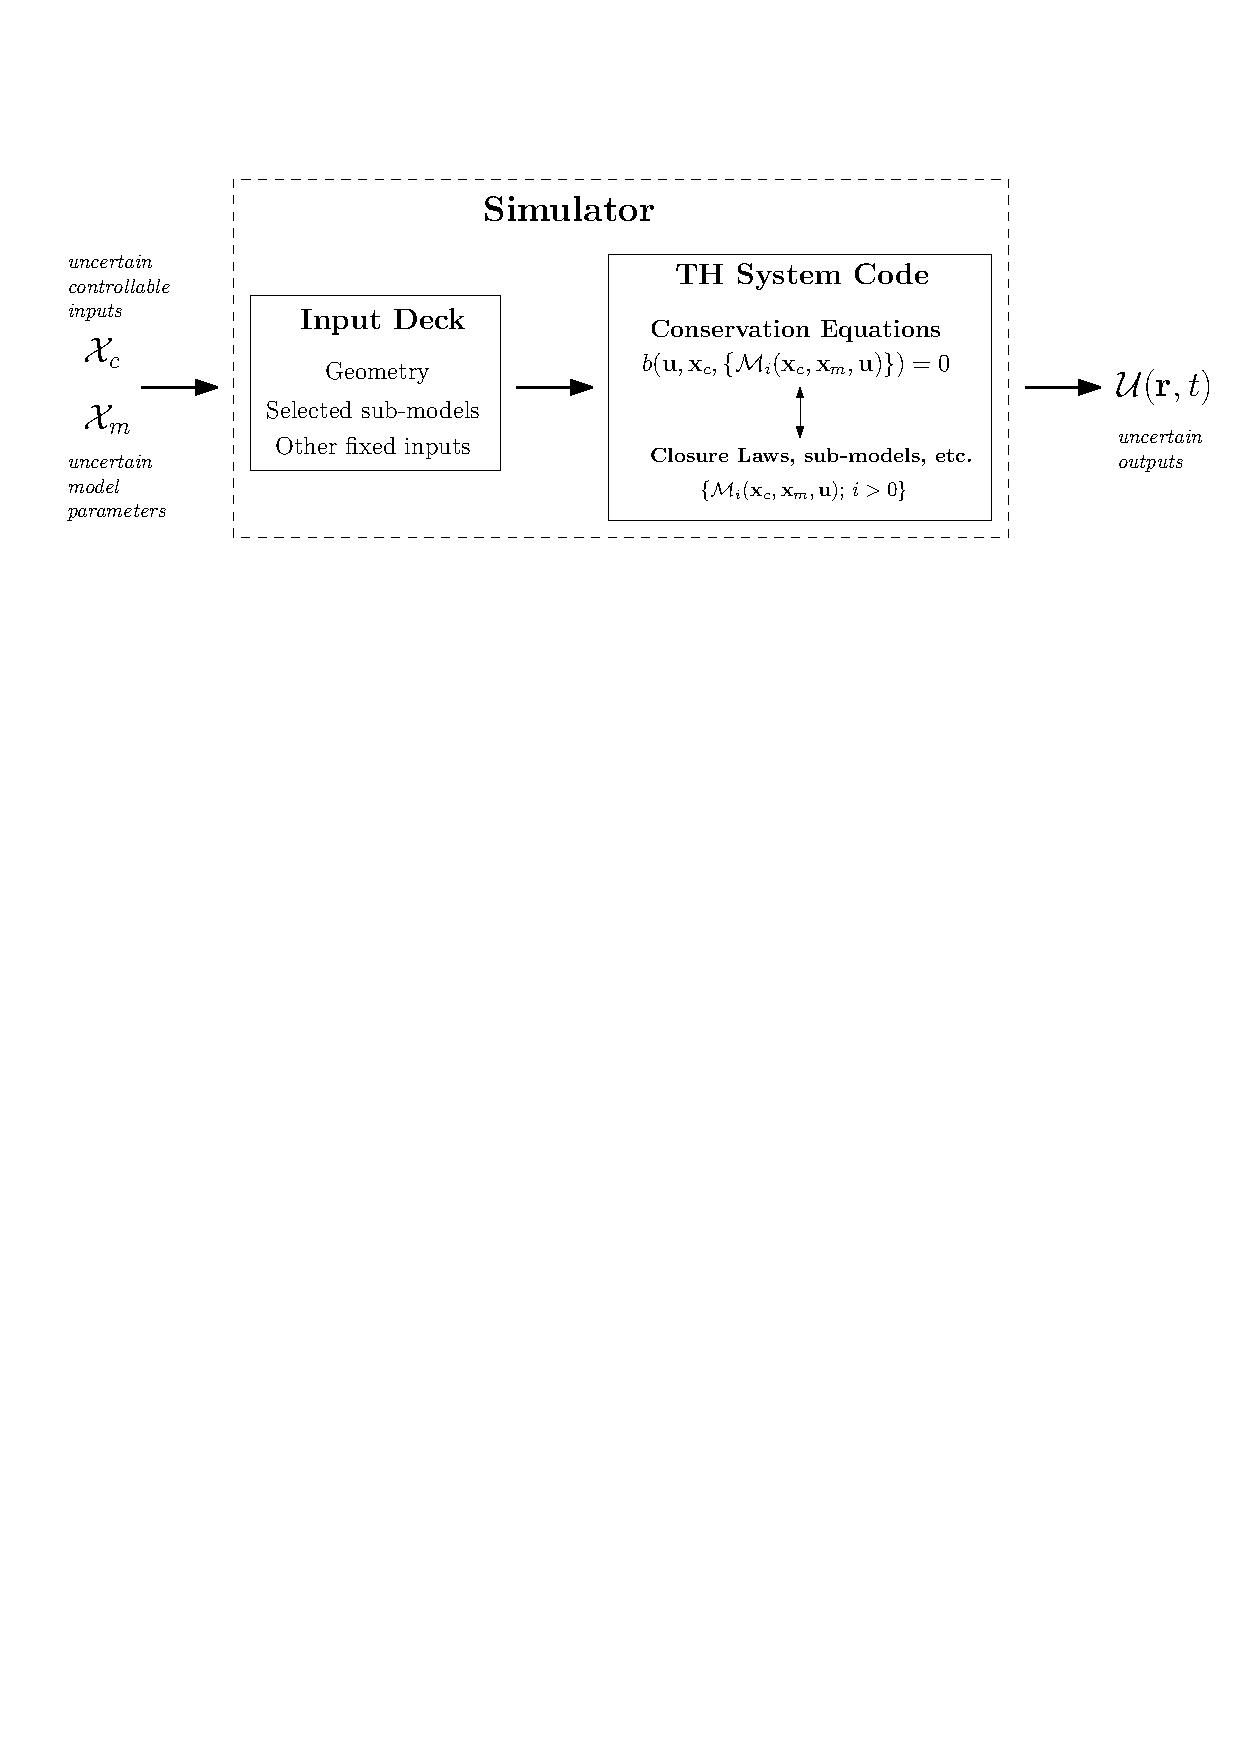
\includegraphics[width=\textwidth]{../figures/chapter1/figures/simulator_uq_forward}
	\caption[Simplified flowchart of forward uncertainty quantification of a simulator prediction.]{Simplified flowchart of forward uncertainty quantification of a simulator prediction. Notice that the simulator has been parametrized by the controllable inputs and physical model parameters, each of which are represented as a random variable.}
	\label{fig:ch1_simulator_uq_forward}
\end{figure}

%-------------------------------------------------------------------------------------
\subsection{Inverse (Backward) Uncertainty Quantification}\label{sub:intro_uq_inverse}
%-------------------------------------------------------------------------------------

% Model parameters
A lot has been said about the origin of the uncertainty associated with the controllable inputs.
The physical model parameters, however, are conceptually different.
\marginpar{Model parameters}
The physical models referred to in this thesis are usually represented either in the form of correlations, phenomenological models, or a mixed between the two (see Section~\ref{sub:intro_th_system_code}).
Therefore, the model parameters do not necessarily have a physical meaning (see Chapter~\ref{ch:bayesian_calibration}) and the source of their uncertainties vary with the type of model.
For instance, in an empirical model the model parameters are the curve-fitting parameters and their uncertainties are observable and can be associated with the dispersion of the data.

% Representativity for NPP application
However, many physical models, be it empirical or mechanistic, are originally derived from experiments on simple systems that do not, strictly speaking, reflect the flow conditions in an \gls[hyper=false]{lwr} (e.g., heated tube vs. rod bundle, low pressure vs. high pressure, etc.) \cite{Bestion2008}.
\marginpar{Separate Effect Test Facilities (SETFs)}
Thus, to better represent the flow characteristics in reactor transient,
experiments with well-specified conditions are conducted in \glspl[hyper=false]{setf}.

These are facilities aimed at reproducing a particular safety-relevant phenomena during transient at a particular part of the reactor \cite{DAuria2012} and their data are used to assess the physical models.
In the assessment,
\marginpar{Calibration against SETFs}
some parameters in the models are adjusted to match the experimental data \cite{Barre1990}.
Alternatively, additional free parameters can also be introduced in the models to serve the same purpose \cite{Bestion2008}.
That is, the parameters are tuning parameters and become measures of the models inadequacy in reproducing the data.
Ultimately, optimal values for the parameters are estimated and implemented in the code.

% Origin of uncertainty
In light of this, it can be argued that the uncertainty associated with the tuning parameters stems from the fact that the calibration was conducted only on limited set of data obtained from selected \glspl[hyper=false]{setf}.
Different \glspl[hyper=false]{setf} for the same phenomena exist, covering wide ranges of flow configurations and experimental boundary conditions.
It is fair to ask if the calibrated value will hold if the calibration were to be conducted on other \glspl[hyper=false]{setf} data for the same phenomena.
Additionally, as tuning parameters, expert-judgment is also often used to estimate the uncertainty.
Experts fixed the range of variation of the parameters based on their expectation of the model performance.

% Inverse uncertainty
To derive the uncertainty associated with the model parameters described above,
the problem can be posed as an inverse problem.
\marginpar{An inverse problem}
In this setting, given a set of experimental data $\{\mathbf{D}\}$ taken with known controllable inputs $\mathbf{x}_c$, the task is then to infer the value of the \emph{unobserved} parameters in the physical model used to predict the same quantity as the experimental data.
To avoid excessive bias to the calibration data, it is important here to acknowledge the observation errors of the experimental data and the controllable inputs, and the possible systematic bias of the associated models.

% Bayesian framework
In a probabilistic setting, a way to make an inference of unobserved parameters based on observed data is
\marginpar{Inverse uncertainty quantification}
through the Bayes' theorem,
\begin{equation*}
	p(\bm{x}_m\,|\,\{\mathbf{D}\},\mathbf{x}_c) = \frac{p(\{\mathbf{D}\}\,|\,\bm{x}_m, \mathbf{x}_c) \cdot p(\bm{x}_m)}{\int p(\{\mathbf{D}\}\,|\,\bm{x}_m, \mathbf{x}_c) \cdot p(\bm{x}_m)\,d\bm{x}_m}
\end{equation*}
where the left-hand side of the equation is the posterior probability density conditioned on the observed data $\{\mathbf{D}\}$ and controllable inputs $\mathbf{x}_c$.
The right-hand side constitutes of the likelihood function $p(\{\mathbf{D}\}\,|\,\bm{x}_m, \mathbf{x}_c)$ (probability of observing data given the parameters), the prior of the model parameters $p(\bm{x}_m)$ (the initial state of knowledge regarding the parameters values before observing the data),
while the denominator is a normalizing constant such that the posterior is a valid \gls[hyper=false]{pdf} (that is, it integrates to one)\footnote{Note that the formulation assumes the controllable inputs $\mathbf{x}_c$ are fully known. If they are considered uncertain, such as due to their inherent variability, then a prior probability can be put on them as well.}.
The posterior represents the knowledge one has on the model parameters values conditioned on the data under the modeling assumption.
Fig.~\ref{fig:ch1_simulator_uq_inverse} depicts a simplified flowchart of the inverse quantification.
\bigfigure[pos=tbhp,
           opt={width=1.0\textwidth},
           label={fig:ch1_simulator_uq_inverse},
           shortcaption={Simplified flowchart of inverse uncertainty quantification of model parameters.}]
{../figures/chapter1/figures/simulator_uq_inverse}
{Simplified flowchart of inverse quantification for model parameters of a simulator.}

The formulation and computation of the posterior above can be seen as a calibration exercise.
That is, it seeks to adjust the model parameters such that the predictions of the simulator are consistent with the observed data (i.e., calibration data) under the assumed likelihood and the prior.
\marginpar{Statistical calibration}
However, instead of obtaining a single estimated value (or values in case of multiple parameters), the resulting posterior is a \gls[hyper=false]{pdf}, conditioned on the observed data.
In relation to the aforementioned expert-judgment for estimating the parameters uncertainty, the approach uses the experimental data to better inform the prior expectation about the model parameters values.
The posterior \gls[hyper=false]{pdf}, in turn, can be used in uncertainty propagation to quantify the uncertainty on the prediction made outside the calibration data set.

% Connection to PREMIUM Benchmark
The importance of characterizing the uncertainty in the physical models parameters was acknowledged by the \gls[hyper=false]{wgama} of the \gls[hyper=false]{oecd}/\gls[hyper=false]{nea}.
This led to the \gls[hyper=false]{premium} project.
Its main goal is to report the state-of-the-art methodologies to quantify the uncertainty in the physical models parameters.
The following will briefly describe the project and highlight the selected main lessons learned from the author's perspective through his participation on behalf of the \glsfirst[hyper=false]{psi} \cite{Wicaksono2016a}.

%-------------------------------------------------------------
\subsection{OECD/NEA PREMIUM project}\label{sub:intro_premium}
%-------------------------------------------------------------

% Introductory paragraph
The \gls[hyper=false]{premium} project was an activity launched by the \gls[hyper=false]{oecd}/\gls[hyper=false]{nea} with the aim to advance the methods for quantifying the uncertainties associated with the physical model parameters in \gls[hyper=false]{th} system codes.
It was the continuation of the project \gls[hyper=false]{bemuse}, which concentrated on the propagation and sensitivity analysis of the input uncertainties in large scale simulation (\gls[hyper=false]{lbloca}).
The main finding of \gls[hyper=false]{bemuse} can be found in \cite{Perez2011}.
The emphasis of the \gls[hyper=false]{premium} benchmark was placed on the derivation of the model parameters uncertainties and their validation.

% Scope of the Project
The scope of the project was limited to the simulation of the phenomenon of core reflood and quenching under conditions representative of a \gls[hyper=false]{pwr} large break \gls[hyper=false]{loca}.
Experimental data from two \glspl[hyper=false]{setf} was made available for the purpose of uncertainty quantification of the model parameters as well as validation.
For the model parameters uncertainty quantification, the data from the \gls[hyper=false]{feba} reflood facility was used.
The derived uncertainties were then propagated and compared with the experimental data from other experimental runs of \gls[hyper=false]{feba} and from another reflood facility (PERICLES).
Thus the main goal of the project followed the approach of statistical uncertainty analyses explained above.

% Phase
Sixteen organizations from $11$ different countries participated in the $4$-year project ($2012$--$2016$) using $6$ different \gls[hyper=false]{th} system codes.
Each participant employing a chosen simulation code and methodology had to contribute to the $5$ following phases of the benchmark:
\begin{enumerate}
	\item \textsc{Phase 1}: Description of the selected simulation code and methodology.
  \item \textsc{Phase 2}: Identification of the uncertain parameters that are most relevant to \gls[hyper=false]{pwr} \gls[hyper=false]{loca} reflooding simulations.
  \item \textsc{Phase 3}: Quantification of the uncertainties in the parameters, using available data from the \gls[hyper=false]{feba} experiment.
  \item \textsc{Phase 4}: Propagation of the quantified uncertainties as part of a blind benchmark exercise based on data from the PERICLES experiment.
  \item \textsc{Phase 5}: Contribution to the analysis and synthesis of the benchmark results.
\end{enumerate}
During the course of the project, three \gls[hyper=false]{oecd}/\gls[hyper=false]{nea} reports have been published \cite{Kovtonyuk2015, Reventos2016,Sanz2017}.
Details can be found in the reports.
The following will describe briefly some of the lessons learned from \gls[hyper=false]{premium} of relevance to the present study.

% Lessons learned
\gls[hyper=false]{premium} provided state-of-the-art (as of $2015$) uncertainty quantification methods for \gls[hyper=false]{th} system codes.
It emphasized methodological issues that are yet to be overcome.
Some of these issues, such as the identification of important parameters, extrapolation of quantified results, scaling, and nodalization were already raised in the $1994$ review studies on uncertainty methods for \gls[hyper=false]{th} codes sponsored by the European Commission \cite{Forge1994}.
At the conclusion of \gls[hyper=false]{premium}, these issues are still considered open problems.

% The problem of systematic identification of important parameters
First, there was an apparent lack of consensus among participants (and thus, the community) for a systematic identification of important parameters in \gls[hyper=false]{th} simulation models.
\marginpar{Identification of important parameters}
Guidelines were indeed provided, but each participant eventually came up with their own selection criteria and methodology, some still relied solely on graph comparison of outputs when changing one parameter at a time \cite{Kovtonyuk2015}.

Although complete exclusion of expert judgment is not feasible (nor advised), it is useful to take benefit from the progress made in the computer experiment community.
For instance, the Morris screening method can be useful in the initial parameter identification and importance ranking process by making the analysis more systematic and robust.
The method can provide smooth transition from the more familiar one-at-a-time method adopted by most participants.
Furthermore, there was a valid issue raised by a participant regarding the possibility of ``complicated'' code response from simultaneous parameters perturbation \cite{Wicaksono2015}.
This can be interpreted as parameter interaction in the literature.
In this case, \gls[hyper=false]{gsa} methods can help in the investigation about its presence. 

% The problem of calibration and overfitting
Secondly, there was a slight disagreement between participants regarding the use of \emph{calibrated parameter}.
This notion stemmed from the use of a Bayesian method (the so-called CIRC\'E \cite{Crecy2001,Reventos2016}, a method based on maximum likelihood approach under linear assumption coupled with normal prior for the parameter) to update the prior distribution of the model parameter such that the resulting posterior distribution yields the closest agreement with the experimental data.
\marginpar{Calibrated parameter and best-estimate code}
In the application of CIRC\'E, the nominal value of the model parameter was allowed to shift following the updated central measure of the posterior.
Such practice of calibration was questioned because the best-estimate code used was, in fact, already calibrated on the basis of larger experimental databases over decades of verification and validation (V\&V) activities.
In other words, the calibration over a very limited set of the \gls[hyper=false]{feba} tests would undermine the built-in (calibrated) models already in place.

That is a valid point of contention.
The results of applying CIRC\'E were mixed. 
On one hand the experimental data from the \gls[hyper=false]{feba} experiment allowed CIRC\'E to reduce the initial uncertainty on the parameters and simultaneously improved the nominal case predictions.
On the other hand, when the updated parameters were used in the uncertainty propagation of another \gls[hyper=false]{feba} test, the narrow uncertainty band on the predictions failed to cover some part of the experimental data.
Moreover, when the same updated parameters were used in the blind uncertainty propagation for another facility there results were poor: poor nominal case prediction and too narrow uncertainty without covering the experimental data \cite{Wicaksono2016a,Sanz2017}.

This indicated a symptom of \emph{overfitting} in which the uncertain parameters were calibrated strongly on one data set and thus became very sensitive to a change of data set.
\marginpar{Overfitting and extrapolation}
The narrow uncertainty obtained indicates that the calibration procedure converged to a ``wrong'' values and thus was not applicable to extrapolation.

While the Bayesian approach makes sense for parameter calibration, updating its value in light of new data,
its application might require accounting for additional sources of uncertainty.
It also makes sense to acknowledge the extensive V\&V activities that serve as the basis of \gls[hyper=false]{th} system codes;
observing one additional data set should not render previous results invalid right away.
Thus it remains an open question how to compromise between learning from new data and preserving what has been learned before.

% The use of metamodel
Finally, there was a natural reluctance among the participants to embrace more recent methods requiring less assumptions (e.g., normal prior of the parameters, linearity between outputs and parameters, etc.) but requiring more code runs.
\marginpar{The use of metamodel}
The use of metamodel can help in alleviating such computational restriction\footnote{It is not, however, cost-free as will be explained in more detail in Chapter~\ref{ch:gp_metamodel}.}, insofar that the error incurred by the use of metamodel can be accepted.
Strictly speaking, the community is not unfamiliar with the use of metamodel (a fast approximating function as a substitute of running the code) for uncertainty analysis, especially in the context of uncertainty propagation\footnote{It was initially used for the estimation of \gls[hyper=false]{pct} probability distribution from uncertainty propagation in the context of safety margin evaluation of \gls[hyper=false]{lbloca} scenario \cite{Boyack1990}.}.
However, in the context of inverse uncertainty quantification, none of the participant took the benefit of using metamodel and relaxed some of the assumptions in calibration.
